
\newcommand{\DynkinAn}{
  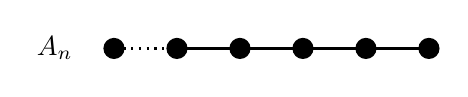
\begin{tikzpicture}[scale=.4]
    \draw (-1,0) node[anchor=east]  {$A_n$};
    \foreach \x in {0,...,5}
    \draw[xshift=\x cm,thick,fill=black] (\x cm,0) circle (.3cm);
    \draw[dotted,thick] (0.3 cm,0) -- +(1.4 cm,0);
    \foreach \y in {1.15,...,4.15}
    \draw[xshift=\y cm,thick] (\y cm,0) -- +(1.4 cm,0);
  \end{tikzpicture}
}

\newcommand{\DynkinAa}{
  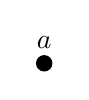
\begin{tikzpicture}[scale=.3]
    \draw (0,0.2) node[anchor=south] {$a$};
    \foreach \x in {0}
    \draw[xshift=\x cm,thick,fill=black] (\x cm,0) circle (.3cm);
  \end{tikzpicture}
}

\newcommand{\DynkinAab}{
  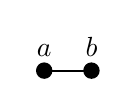
\begin{tikzpicture}[scale=.3]
    \draw (0,0.2) node[anchor=south] {$a$};
    \draw (2,0.2) node[anchor=south] {$b$};
    \foreach \x in {0,1}
    \draw[xshift=\x cm,thick,fill=black] (\x cm,0) circle (.3cm);
    \foreach \y in {0.15,...,0.15}
    \draw[xshift=\y cm,thick] (\y cm,0) -- +(1.4 cm,0);
  \end{tikzpicture}
}

\newcommand{\DynkinAabc}{
  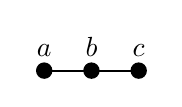
\begin{tikzpicture}[scale=.3]
    \draw (0,0.2) node[anchor=south] {$a$};
    \draw (2,0.2) node[anchor=south] {$b$};
    \draw (4,0.2) node[anchor=south] {$c$};
    \foreach \x in {0,1,2}
    \draw[xshift=\x cm,thick,fill=black] (\x cm,0) circle (.3cm);
    \foreach \y in {0.15,...,1.15}
    \draw[xshift=\y cm,thick] (\y cm,0) -- +(1.4 cm,0);
  \end{tikzpicture}
}

\newcommand{\DynkinAabcd}{
  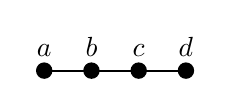
\begin{tikzpicture}[scale=.3]
    \draw (0,0.2) node[anchor=south] {$a$};
    \draw (2,0.2) node[anchor=south] {$b$};
    \draw (4,0.2) node[anchor=south] {$c$};
    \draw (6,0.2) node[anchor=south] {$d$};
    \foreach \x in {0,1,2,3}
    \draw[xshift=\x cm,thick,fill=black] (\x cm,0) circle (.3cm);
    \foreach \y in {0.15,...,2.15}
    \draw[xshift=\y cm,thick] (\y cm,0) -- +(1.4 cm,0);
  \end{tikzpicture}
}


\newcommand{\DynkinBn}{
  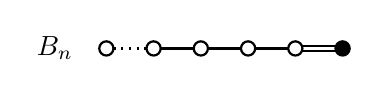
\begin{tikzpicture}[scale=.3]
    \draw (-1,0) node[anchor=east]  {$B_n$};
    \foreach \x in {0,...,4}
    \draw[xshift=\x cm,thick] (\x cm,0) circle (.3cm);
    \draw[xshift=5 cm,thick,fill=black] (5 cm, 0) circle (.3 cm);
    \draw[dotted,thick] (0.3 cm,0) -- +(1.4 cm,0);
    \foreach \y in {1.15,...,3.15}
    \draw[xshift=\y cm,thick] (\y cm,0) -- +(1.4 cm,0);
    \draw[thick] (8.3 cm, .1 cm) -- +(1.4 cm,0);
    \draw[thick] (8.3 cm, -.1 cm) -- +(1.4 cm,0);
  \end{tikzpicture}
}

\newcommand{\DynkinBab}{
  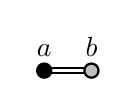
\begin{tikzpicture}[scale=.3]
    \draw (0,0.2) node[anchor=south] {$a$};
    \draw (2,0.2) node[anchor=south] {$b$};
    \foreach \x in {0}
    \draw[xshift=\x cm,thick,fill=black] (\x cm,0) circle (.3cm);
    \foreach \x in {1}
    \draw[xshift=\x cm,thick,fill=lightgray] (\x cm,0) circle (.3cm);
    \foreach \y in {0.15,...,0.15}
    \draw[xshift=\y cm,thick] (\y cm,+0.1 cm) -- +(1.4 cm,0);
    \foreach \y in {0.15,...,0.15}
    \draw[xshift=\y cm,thick] (\y cm,-0.1 cm) -- +(1.4 cm,0);
  \end{tikzpicture}
}

\newcommand{\DynkinBabc}{
  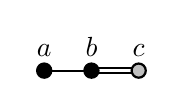
\begin{tikzpicture}[scale=.3]
    \draw (0,0.2) node[anchor=south] {$a$};
    \draw (2,0.2) node[anchor=south] {$b$};
    \draw (4,0.2) node[anchor=south] {$c$};
    \foreach \x in {0,1}
    \draw[xshift=\x cm,thick,fill=black] (\x cm,0) circle (.3cm);
    \foreach \x in {2}
    \draw[xshift=\x cm,thick,fill=lightgray] (\x cm,0) circle (.3cm);
    \foreach \y in {0.15,...,0.15}
    \draw[xshift=\y cm,thick] (\y cm,0) -- +(1.4 cm,0);
    \foreach \y in {1.15,...,1.15}
    \draw[xshift=\y cm,thick] (\y cm,+0.1 cm) -- +(1.4 cm,0);
    \foreach \y in {1.15,...,1.15}
    \draw[xshift=\y cm,thick] (\y cm,-0.1 cm) -- +(1.4 cm,0);
  \end{tikzpicture}
}


\newcommand{\DynkinCn}{
  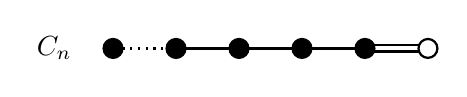
\begin{tikzpicture}[scale=.4]
    \draw (-1,0) node[anchor=east]  {$C_n$};
    \foreach \x in {0,...,4}
    \draw[xshift=\x cm,thick,fill=black] (\x cm,0) circle (.3cm);
    \draw[xshift=5 cm,thick] (5 cm, 0) circle (.3 cm);
    \draw[dotted,thick] (0.3 cm,0) -- +(1.4 cm,0);
    \foreach \y in {1.15,...,3.15}
    \draw[xshift=\y cm,thick] (\y cm,0) -- +(1.4 cm,0);
    \draw[thick] (8.3 cm, .1 cm) -- +(1.4 cm,0);
    \draw[thick] (8.3 cm, -.1 cm) -- +(1.4 cm,0);
  \end{tikzpicture}
}

\newcommand{\DynkinCab}{
  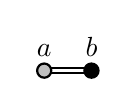
\begin{tikzpicture}[scale=.3]
    \draw (0,0.2) node[anchor=south] {$a$};
    \draw (2,0.2) node[anchor=south] {$b$};
    \foreach \x in {0}
    \draw[xshift=\x cm,thick,fill=lightgray] (\x cm,0) circle (.3cm);
    \foreach \x in {1}
    \draw[xshift=\x cm,thick,fill=black] (\x cm,0) circle (.3cm);
    \foreach \y in {0.15,...,0.15}
    \draw[xshift=\y cm,thick] (\y cm,+0.1 cm) -- +(1.4 cm,0);
    \foreach \y in {0.15,...,0.15}
    \draw[xshift=\y cm,thick] (\y cm,-0.1 cm) -- +(1.4 cm,0);
  \end{tikzpicture}
}

\newcommand{\DynkinCabc}{
  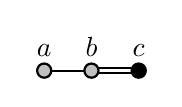
\begin{tikzpicture}[scale=.3]
    \draw (0,0.2) node[anchor=south] {$a$};
    \draw (2,0.2) node[anchor=south] {$b$};
    \draw (4,0.2) node[anchor=south] {$c$};
    \foreach \x in {0,1}
    \draw[xshift=\x cm,thick,fill=lightgray] (\x cm,0) circle (.3cm);
    \foreach \x in {2}
    \draw[xshift=\x cm,thick,fill=black] (\x cm,0) circle (.3cm);
    \foreach \y in {0.15,...,0.15}
    \draw[xshift=\y cm,thick] (\y cm,0) -- +(1.4 cm,0);
    \foreach \y in {1.15,...,1.15}
    \draw[xshift=\y cm,thick] (\y cm,+0.1 cm) -- +(1.4 cm,0);
    \foreach \y in {1.15,...,1.15}
    \draw[xshift=\y cm,thick] (\y cm,-0.1 cm) -- +(1.4 cm,0);
  \end{tikzpicture}
}


\newcommand{\DynkinDn}{
  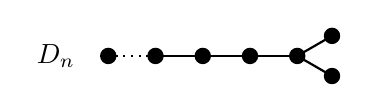
\begin{tikzpicture}[scale=.3]
    \draw (-1,0) node[anchor=east]  {$D_n$};
    \foreach \x in {0,...,4}
    \draw[xshift=\x cm,thick,fill=black] (\x cm,0) circle (.3cm);
    \draw[xshift=8 cm,thick,fill=black] (30: 17 mm) circle (.3cm);
    \draw[xshift=8 cm,thick,fill=black] (-30: 17 mm) circle (.3cm);
    \draw[dotted,thick] (0.3 cm,0) -- +(1.4 cm,0);
    \foreach \y in {1.15,...,3.15}
    \draw[xshift=\y cm,thick] (\y cm,0) -- +(1.4 cm,0);
    \draw[xshift=8 cm,thick] (30: 3 mm) -- (30: 14 mm);
    \draw[xshift=8 cm,thick] (-30: 3 mm) -- (-30: 14 mm);
  \end{tikzpicture}}

\newcommand{\DynkinGtwo}{
  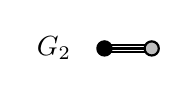
\begin{tikzpicture}[scale=.3]
    \draw (-1,0) node[anchor=east]  {$G_2$};
    \draw[thick,fill=black] (0 ,0) circle (.3 cm);
    \draw[thick,fill=lightgray] (2 cm,0) circle (.3 cm);
    \draw[thick] (30: 3mm) -- +(1.5 cm, 0);
    \draw[thick] (0: 3 mm) -- +(1.4 cm, 0);
    \draw[thick] (-30: 3 mm) -- +(1.5 cm, 0);
  \end{tikzpicture}}

\newcommand{\DynkinFfour}{
  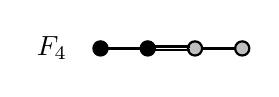
\begin{tikzpicture}[scale=.3]
    \draw (-3,0) node[anchor=east]  {$F_4$};
    \draw[thick,fill=black] (-2 cm ,0) circle (.3 cm);
    \draw[thick,fill=black] (0 ,0) circle (.3 cm);
    \draw[thick,fill=lightgray] (2 cm,0) circle (.3 cm);
    \draw[thick,fill=lightgray] (4 cm,0) circle (.3 cm);
    \draw[thick] (15: 3mm) -- +(1.5 cm, 0);
    \draw[xshift=-2 cm,thick] (0: 3 mm) -- +(1.4 cm, 0);
    \draw[thick] (-15: 3 mm) -- +(1.5 cm, 0);
    \draw[xshift=2 cm,thick] (0: 3 mm) -- +(1.4 cm, 0);
  \end{tikzpicture}}

\newcommand{\DynkinEsix}{
  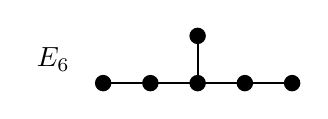
\begin{tikzpicture}[scale=.3]
    \draw (-1,1) node[anchor=east]  {$E_6$};
    \foreach \x in {0,...,4}
    \draw[thick,fill=black,xshift=\x cm] (\x cm,0) circle (3 mm);
    \foreach \y in {0,...,3}
    \draw[thick,xshift=\y cm] (\y cm,0) ++(.3 cm, 0) -- +(14 mm,0);
    \draw[thick,fill=black] (4 cm,2 cm) circle (3 mm);
    \draw[thick] (4 cm, 3mm) -- +(0, 1.4 cm);
  \end{tikzpicture}}

\newcommand{\DynkinEseven}{
  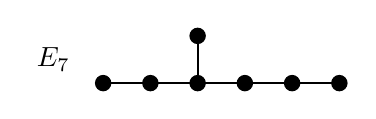
\begin{tikzpicture}[scale=.3]
    \draw (-1,1) node[anchor=east]  {$E_7$};
    \foreach \x in {0,...,5}
    \draw[thick,fill=black,xshift=\x cm] (\x cm,0) circle (3 mm);
    \foreach \y in {0,...,4}
    \draw[thick,xshift=\y cm] (\y cm,0) ++(.3 cm, 0) -- +(14 mm,0);
    \draw[thick,fill=black] (4 cm,2 cm) circle (3 mm);
    \draw[thick] (4 cm, 3mm) -- +(0, 1.4 cm);
  \end{tikzpicture}}

\newcommand{\DynkinEeight}{
  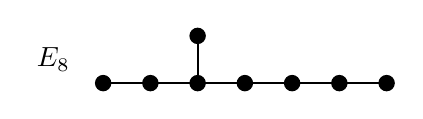
\begin{tikzpicture}[scale=.3]
    \draw (-1,1) node[anchor=east]  {$E_8$};
    \foreach \x in {0,...,6}
    \draw[thick,fill=black,xshift=\x cm] (\x cm,0) circle (3 mm);
    \foreach \y in {0,...,5}
    \draw[thick,xshift=\y cm] (\y cm,0) ++(.3 cm, 0) -- +(14 mm,0);
    \draw[thick,fill=black] (4 cm,2 cm) circle (3 mm);
    \draw[thick] (4 cm, 3mm) -- +(0, 1.4 cm);
  \end{tikzpicture}}

